%Übersicht ist in getrennter Datei 3d-uebersicht.
\paragraph{Vertiefung}
\label{3d:vertiefung}
\begin{wrapfigure}{r}{0.42\textwidth}
  \begin{center}
    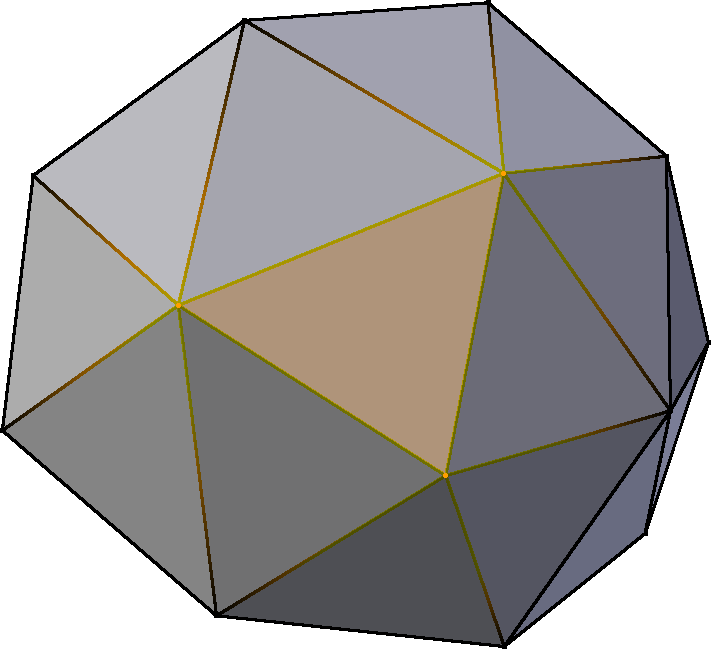
\includegraphics[width=0.42\textwidth]{bilder/3D_VerticesPolygone}
  \end{center}
  \caption{Die gelb markierten Eckpunkte beschreiben das hervorgehobene Dreieck in dem 3D-Modell.}
\end{wrapfigure}
Ein übliches 3D-Modell besteht aus Eckpunkten (\emph{vertices}), die Polygone beschreiben. Meistens handelt es sich dabei um Dreiecke. Sind die Eckpunkte und die zu den Polygonen gehörenden Kanten erfasst, spricht man von einem Drahtgittermodell (\emph{wire-frame model} oder \emph{mesh}). Sind nur die Eckpunkte erfasst, handelt es sich um eine Punktwolke, welche beispielsweise von 3D-Scannern erzeugt wird. Um eine Punktwolke weiter zu verarbeiten, muss diese vorher meist in ein Drahtgittermodell umgewandelt werden.

Die Inhalte von 3D-Modellen können in drei Kategorien eingeteilt werden: Geometrie, Oberflächeneigenschaften sowie Belichtungs- und Kameraparameter. Zusätzlich kann noch eine Animation oder eine Interaktion hinterlegt sein. Aus diesen Angaben wird die Visualisierung berechnet. Dieser Vorgang wird als Bildsynthese bezeichnet (\emph{rendering}) und resultiert in statischen Rastergrafiken, Videos oder interaktive Modelle.

\begin{figure}[h!tb]
  \begin{center}
    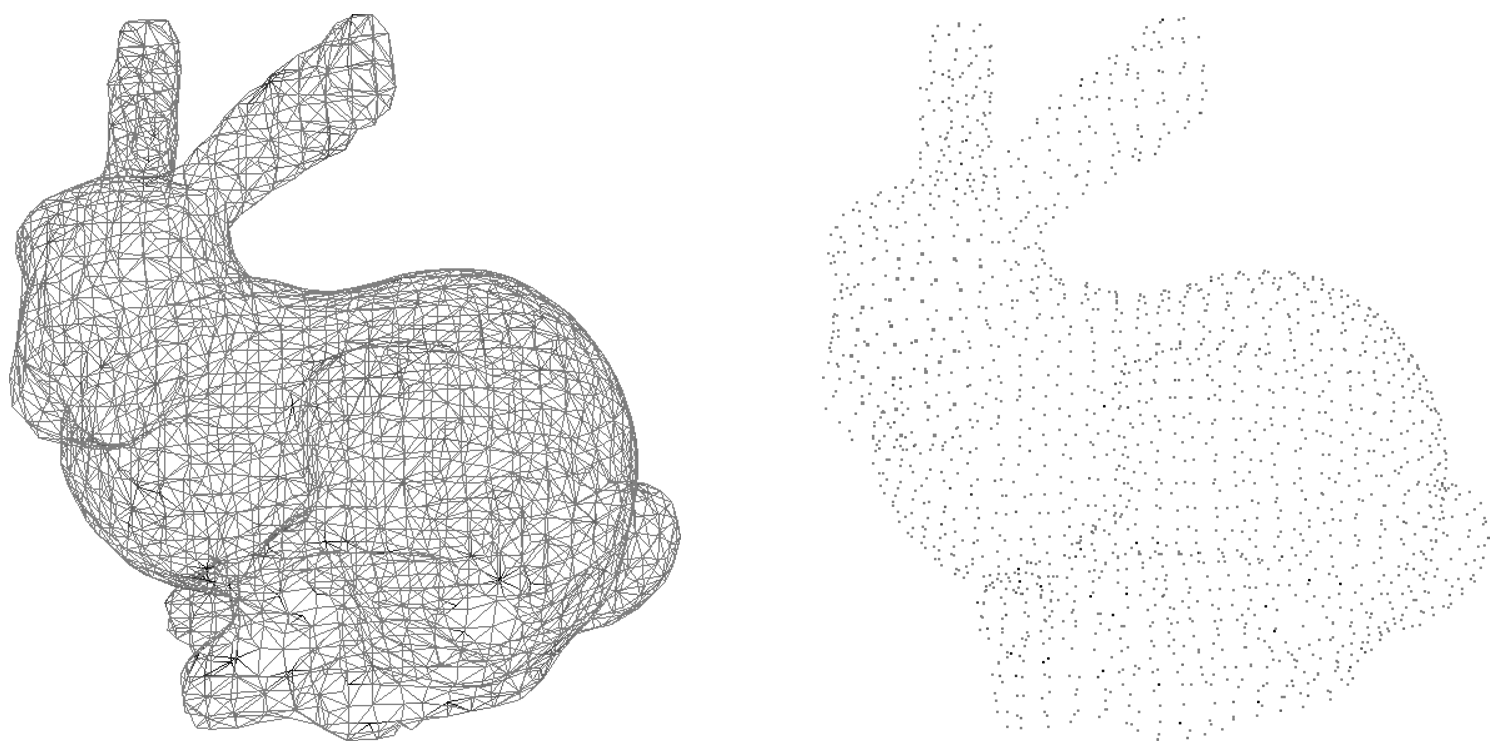
\includegraphics[width=0.75\textwidth]{bilder/3D_DrahtgitterPunktwolke}
  \end{center}
  \caption{Das Stanford Bunny links als Drahtgittermodell und rechts als Punktwolke.}
\end{figure}

\subparagraph{Geometrie} Die Form eines 3D-Modells kann mit vier verschiedenen Methoden beschrieben werden: durch ein Drahtgittermodell oder Facetten, parametrisch mit mathematisch beschriebenen Kurven und Flächen, mittels geometrischen Körpern, der sogenannten Konstruktiven Festkörpergeometrie, oder durch die begrenzenden Oberflächen, dem sogenannten Begrenzungsflächenmodell.

{\bfseries Drahtgittermodell:} Hierbei wird die Form des 3D-Modells durch dessen Eckpunkte beschrieben, welche wiederum eine Reihe von Polygonen bilden, die zusammen die Oberfläche des Modells darstellen. Drahtgittermodelle sind einfach und schnell zu rendern, jedoch sind bei Detailansichten von konkaven oder konvexen Oberflächen immer die Flächen und scharfen Kanten der einzelnen Polygone erkennbar. Mittels sogenannten Shading-Algorithmen kann beim Rendern der Eindruck von gleichmäßigen Oberflächen generiert werden. Jedoch ist dann an der Kontur immer noch die polygonale Herkunft zu erkennen, wie in Abbildung \ref{abb:3D-render} im Abschnitt Oberflächeneigenschaften ab Seite \pageref{3d_aussehen} dargestellt.  

Eine Annäherung an eine gleichmäßige Oberfläche kann auch durch eine größere Anzahl an kleineren Polygonen erzielt werden, was aber zur Folge hat, dass die Dateigröße des Modells wächst. 

{\bfseries Parametrische Darstellung:} Viele Kurven und Flächen können mathematisch mit wenigen Parametern errechnet werden. Im Bereich der 3D-Grafik werden für die parametrische Darstellung häufig NURBS (Non-Uniform Rational B-Splines, nicht-uniforme rationale B-Splines) verwendet. Die Verwendung von mathematisch beschriebenen Kurven und Flächen erlaubt eine in der Detailliertheit der Oberfläche verlustfreie Skalierbarkeit. Wird ein 3D-Modell mit parametrischen Flächen in einem Format gespeichert, das diese nicht unterstützt, muss das Modell in Polygone umgerechnet werden, was dazu führt, dass Informationen der Oberflächenstruktur verloren gehen, was vergleichbar mit dem Informationsverlust bei der Konvertierung von einer Vektorgrafik in eine Rastergrafik ist.

{\bfseries Konstruktive Festkörpergeometrie:} 3D-Modelle können, anstatt durch Eckpunkte, Flächen oder Kurven auch mit Hilfe von geschlossenen geometrischen Körpern konstruiert werden. Dabei kann die Vereinigung, die Differenz oder die Schnittmenge der Körper gebildet werden. Beispielsweise kann ein Verkehrshütchen aus der Vereinigung eines Kegels und eines flachen Quaders konstruiert werden. Daher wird diese Vorgehensweise als Konstruktive Festkörpergeometrie (Constructive Solid Geometry, CSG) bezeichnet. Sie erfordert die Speicherung sowohl der einzelnen geometrischen Körper, als auch der angewendeten Methoden, um eine spätere Bearbeitung der Modelle einfach zu ermöglichen. Insbesondere Dateiformate aus dem CAD-Bereich berücksichtigen dies. Eine Konvertierung von Formaten, die CSG unterstützen, zu denen, die keine unterstützen, führt zu Einschränkungen bei der Bearbeitbarkeit, da nur noch Polygone und deren Eckpunkte verändert werden können. Eine Konvertierung von einem Polygonformat zu einem CSG-Format ist nur schwer möglich. 

{\bfseries Begrenzungsflächenmodell:} Eine weitere Form der Speicherung der Geometrien von 3D-Modellen aus dem CAD-Bereich stellt das Begrenzungsflächenmodell (Boundary Representation, B-Rep) dar. Dabei wird das Modell durch dessen begrenzende Oberflächen beschrieben.


\subparagraph{Oberflächeneigenschaften}\label{3d_aussehen}
Neben der Form müssen für ein 3D-Modell auch Obeflächeneigenschaften gespeichert werden, die das Aussehen des Modells bestimmen. Neben der Farbe gehören dazu Texturen und Materialeigenschaften, die kombiniert zu einem sehr realistisch wirkenden 3D-Modell führen können. 

Jedem Punkt einer Punktwolke oder den Eckpunkten und Polygonen können Farbwerte zugeordnet werden. Texturen können abstrakt als eine auf das Modell aufgebrachte Tapete verstanden werden. Beispielsweise kann auf einen einfachen Zylinder ein Bild von Holzmaserung aufgebracht werden, um einen Baumstamm fotorealistisch darstellen zu können. Dabei wird jedem Punkt im 3D-Modell ein Punkt aus dem zweidimensionalen Bild zugewiesen. 

\begin{figure}
\centering
\begin{subfigure}{.5\textwidth}
  \centering
  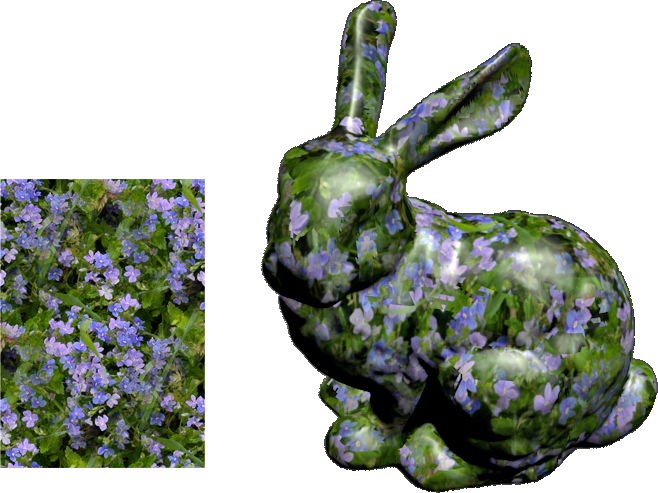
\includegraphics[width=.9\linewidth]{bilder/3D_Textur}
  \caption{}
\end{subfigure}%
\begin{subfigure}{.5\textwidth}
  \centering
  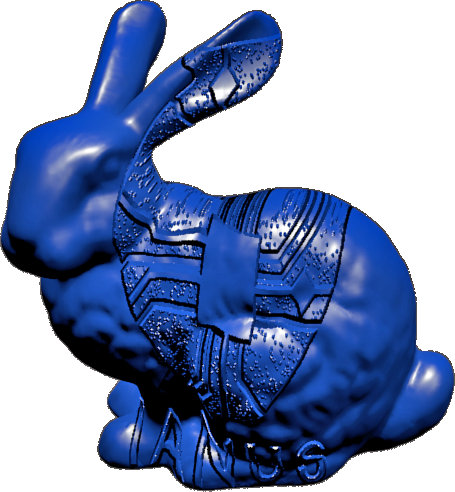
\includegraphics[width=.6\linewidth]{bilder/3D_Bump}
  \caption{}
\end{subfigure}
\caption{(a) Eine Textur und deren Anwendung auf ein 3D-Modell. (b) Mittels Bumpmapping wurde das IANUS-Logo auf ein 3D-Modell aufgebracht. Es erweckt den Anschein einer dreidimensionalen Veränderung der Oberfläche, jedoch hat sich in der Geometrie des Modells nichts verändert, was an den Umrissen zu erkennen ist.}
\end{figure}

Auch die Materialeigenschaften können in einem 3D-Modell modelliert werden, um dem Objekt die gewünschten Reflexionseigenschaften zuzuweisen, denn ein Holztisch weist bei Beleuchtung andere Eigenschaften auf als ein Glastisch. Hierfür werden in dem Modell verschiedene Parameter gespeichert, welche diffuses Streulicht, spiegelndes Spekularlicht, Umgebungslicht, Transparenz, Lichtbrechung, Lichtemission etc. beschreiben.

Eine weitere Technik, um das Aussehen einer Oberfläche zu beeinflussen ist das Bumpmapping. Dabei werden mittels einer Textur die Normalenvektoren der einzelnen Polygone verändert, was dazu führt, dass die Schattierungen und Reflexionen auf der Oberfläche verändert werden und somit Oberflächenunebenheiten simuliert werden, die geometrisch eigentlich nicht vorhanden sind. Weitere Beispiele ähnliche Techniken sind Normal Maps oder Transparency Maps, welche den Schattenwurf, die Reflektion und die Transparenz eines Objektes beeinflussen können. 

Die Oberflächeneigenschaften werden mit Shadern beim Rendern visuell umgesetzt. Shader (dt. Schattierer) sind Programme, die mittels verschiedener Algorithmen unter Berücksichtigung der Lichtquellen die Farbe für jeden darzustellenden Pixel berechnen, um das Aussehen des 3D-Modells in der gerenderten Darstellung zu bestimmen. Ein Shader kann beispielsweise den Eindruck von gleichmäßigen Oberflächen erzeugen, wie in Abbildung \ref{abb:3D-render} dargestellt.

\begin{figure}[!hbt]
  \begin{center}
    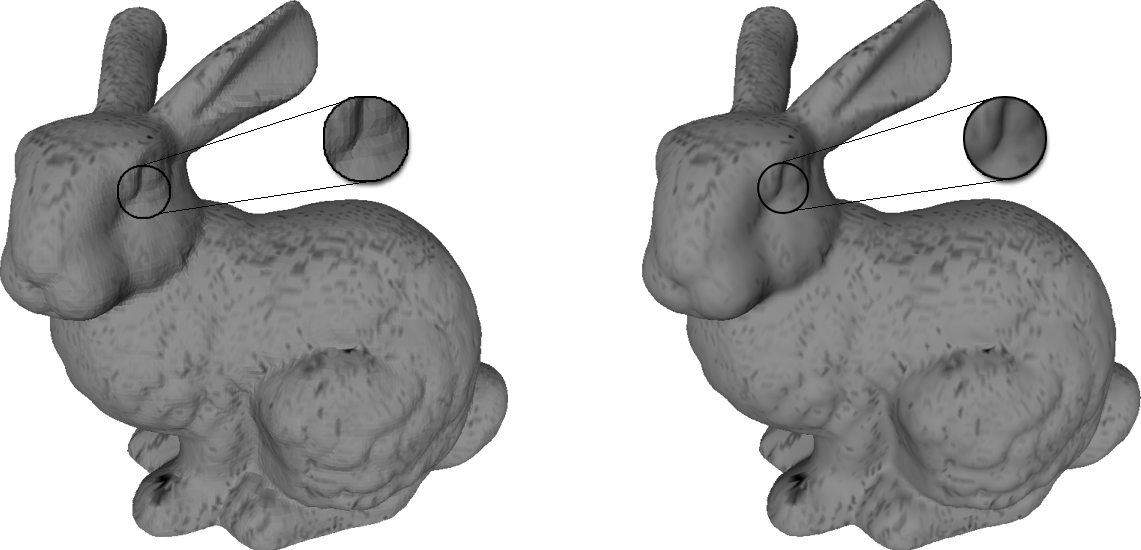
\includegraphics[width=0.8\textwidth]{bilder/3D_Render}
  \end{center}
  \caption{Das linke Modell wurde ohne spezielle Shader gerendert, weshalb die einzelnen Polygone zu erkennen sind. Wird auf das gleiche Modell ein glättender Shader angewendet, entsteht der Eindruck von gleichmäßigen Oberflächen, wie im rechten Teil der Abbildung.}
	\label{abb:3D-render}
\end{figure}


\subparagraph{Belichtungs- und Kameraparameter}
Wie einem Nutzer ein 3D-Modell angezeigt wird, hängt von dem Szenenaufbau ab. Dazu gehören die Größe des Viewports, die Positionierung des 3D-Modells darin, die Position der Kamera und die Lichteinstellungen.

Der Viewport ist dabei vergleichbar mit einer Bühne, die den für die Darstellung zur Verfügung stehenden Bildausschnitt in seiner Höhe, Breite und Tiefe definiert. Für die Kamera muss nicht nur die Position, sondern auch die Blickrichtung gespeichert werden.

Werden 3D-Inhalte ohne Licht gerendert, wird ein schwarzes Bild erzeugt. Daher sind Lichtquellen notwendig, um die Szene auszuleuchten. Werden keine Angaben zu Anzahl, Position, Intensität und Art der Lichtquellen gespeichert, bleibt dies dem Nutzer überlassen oder sie werden gegebenfalls automatisch vom Programm  gesetzt.

Die Szene kann ein oder mehrere Modelle umfassen, welche auch gruppiert werden können. Gruppierungen sind insbesondere dann notwendig, wenn ein Modell aus mehreren Teilen besteht. Dabei muss außerdem die Lage der Teile zueinander gespeichert werden. Es handelt sich dabei um Transformationen, die Verschiebungen, Drehungen oder Skalierungen der Objekte betreffen. 

Bei der Darstellung von umfangreichen Szenen können unterschiedliche Detailstufen für die einzelnen Objekte verwendet werden. Beispielsweise kann eine Mauer im Vordergrund, nahe der Kamera sehr detailliert dargestellt werden, währen ein Baum weit im Hintergrund nur grob angedeutet werden muss, wobei der Detailgrad von 3D-Modellen dabei von der Anzahl der Polygone abhängt. Dieser Detaillierungsgrad wird als "`Level of Detail"' (LOD) bezeichnet und findet insbesondere dann Anwendung, wenn das Rendern von 3D-Modellen effizienter werden soll.

\begin{figure}[!hbt]
  \begin{center}
    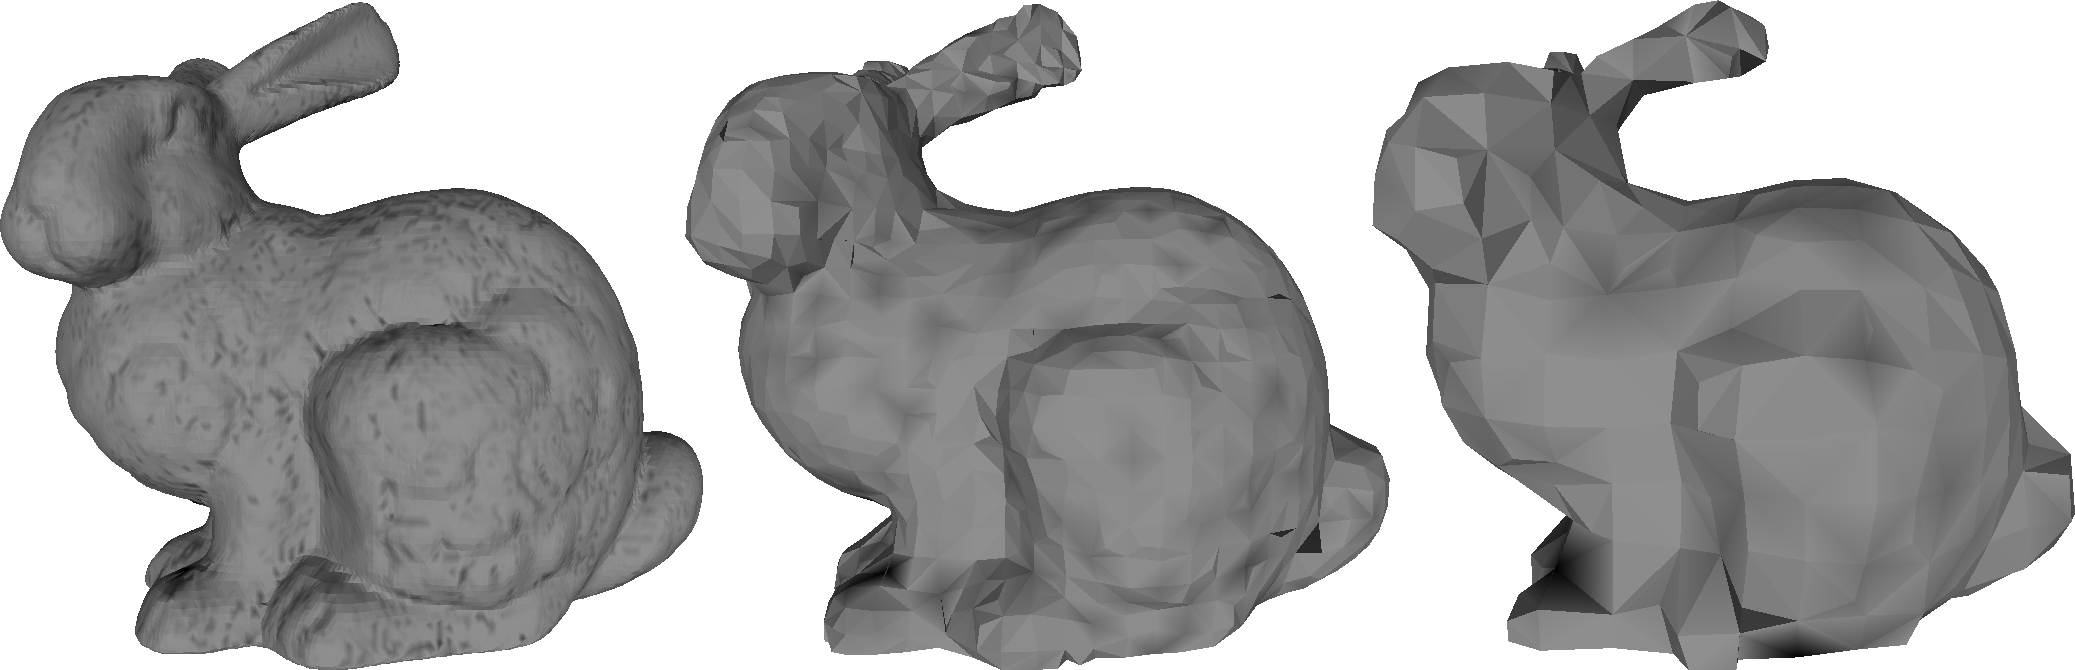
\includegraphics[width=\textwidth]{bilder/3D_LOD}
  \end{center}
  \caption{Auswirkungen von verschiedenen Detaillierungsgraden (LOD) auf ein 3D-Modell. Das Stanford Bunny mit 69451, 3851 und 948 Polygonen.}
\end{figure}


\subparagraph{Animation und Interaktion}
Für Animation und Interaktion ist die Speicherung von zusätzlichen Parametern erforderlich. Dies muss bei der Wahl eines Archivierungsformates berücksichtigt werden und erfordert zusätzliche Angaben in der Dokumentation. Werden Animationen beispielsweise als Videodateien exportiert, sollten die Hinweise in dem Abschnitt Video ab Seite \pageref{video} berücksichtigt werden.


\subparagraph{Speicherung der verschiedenen Eigenschaften}
Nicht jedes 3D"=Format unterstützt die Speicherung aller eben genannten Eigenschaften. Daher muss bei der Wahl des Speicherformates bedacht werden, welche Eigenschaften unbedingt erhalten bleiben sollen. Beispielsweise ist für ein gescanntes Objekt die Speicherung von Lichtquellen oder Animationen nicht unbedingt erforderlich, wohingegen bei einer Architekturrekonstruktion zur Darstellung von Lichtverhältnissen die Lichtquellen unerlässlich sind.

Eine Übersicht über die Speichereigenschaften der hier empfohlenen Formate zur Langzeitarchivierung gibt die folgende Tabelle.\footnote{Nach K. McHenry -- P. Bajcsy, An Overview of 3D Data Content, File Formats and Viewers (2008)}

Die Tabelle ist nicht erschöpfend, da es noch viele weitere spezielle Eigenschaften von 3D-Inhalten gibt, die aber oft nur in spezialisierten, häufig proprietären Anwendungen und 3D-Formaten zum Tragen kommen. Daher ist außerdem zu empfehlen, dass die originalen Dateien ebenfalls archiviert werden, falls es sich dabei nicht schon um eines der hier angegebenen Formate handelt.

\begin{table}[hbt]
\centering
\footnotesize
\begin{tabular}{cccccccccccccc}
	\toprule
	Format	& \multicolumn{4}{c}{Geometrie} & \multicolumn{4}{c}{Aussehen} & \multicolumn{4}{c}{Szene} & Anim.\\
	\cmidrule(lr){2-5}
	\cmidrule(lr){6-9}
	\cmidrule(lr){10-13}
		 & DG & P & CSG & B-Rep & F & X & B & M & V & L & T & G & \\
	\midrule
	X3D & \checkmark & \checkmark & & & \checkmark & \checkmark & \checkmark& \checkmark & \checkmark & \checkmark & \checkmark & \checkmark & \checkmark \\
	\cmidrule(lr){2-5}
	\cmidrule(lr){6-9}
	\cmidrule(lr){10-13}
	COLL. & \checkmark & \checkmark & &\checkmark &\checkmark &\checkmark & \checkmark& \checkmark & \checkmark & \checkmark & \checkmark & \checkmark & \checkmark \\
	\cmidrule(lr){2-5}
	\cmidrule(lr){6-9}
	\cmidrule(lr){10-13}
	OBJ &\checkmark &\checkmark & & &\checkmark &\checkmark &\checkmark &\checkmark & & & &\checkmark &  \\
	\cmidrule(lr){2-5}
	\cmidrule(lr){6-9}
	\cmidrule(lr){10-13}
	PLY &\checkmark & & & &\checkmark &\checkmark &\checkmark &\checkmark & & & & &  \\
	\cmidrule(lr){2-5}
	\cmidrule(lr){6-9}
	\cmidrule(lr){10-13}
	VRML & \checkmark & \checkmark & & & \checkmark & \checkmark & \checkmark& \checkmark & \checkmark & \checkmark & \checkmark & \checkmark & \checkmark \\
	\cmidrule(lr){2-5}
	\cmidrule(lr){6-9}
	\cmidrule(lr){10-13}
	STL &\checkmark & & & &(\checkmark) & & & & & & & &  \\
	\cmidrule(lr){2-5}
	\cmidrule(lr){6-9}
	\cmidrule(lr){10-13}
	DXF &\checkmark &\checkmark &\checkmark &\checkmark &\checkmark & & & & & & &\checkmark &  \\
	\cmidrule(lr){2-5}
	\cmidrule(lr){6-9}
	\cmidrule(lr){10-13}
	U3D & \checkmark & & & & \checkmark & \checkmark & \checkmark& & \checkmark & \checkmark & \checkmark & \checkmark & \checkmark \\
	\cmidrule(lr){2-5}
	\cmidrule(lr){6-9}
	\cmidrule(lr){10-13}
%	STP &\checkmark &\checkmark &\checkmark &\checkmark &\checkmark & & & & & & &\checkmark &  \\
%	\cmidrule(lr){2-5}
%	\cmidrule(lr){6-9}
%	\cmidrule(lr){10-13}
%	IGS &\checkmark &\checkmark &\checkmark &\checkmark &\checkmark & & & & & &\checkmark &\checkmark &   \\
	\bottomrule 
\end{tabular}
\caption{Unterstützte Eigenschaften von verschiedenen 3D-Formaten. DG~= Drahtgittermodell, P~= Parametrisch, F~= Farbe, X~= Textur mittels Bild, B~= Bumpmapping, M~= Material, V~= Viewport und Kamera, L~= Lichtquellen, T~= Transformationen, G~= Gruppierung. Leere Zellen bedeuten entweder fehlende Speichereigenschaften oder es wurden keine Angaben in der jeweiligen Formatspezifikation gefunden.}
\label{tab:3Deigenschaften}
\end{table}

\paragraph{Praxis}
Im Umgang mit 3D-Inhalten müssen in der Praxis einige Details beachtet werden. Dazu gehören die Hinweise aus der Londoner Charta und dass bei der Konvertierung von einem Format in ein anderes Informationsverlust auftreten kann. Die Weitergabe von 3D-Modellen kann mittels verschiedenen Portalen oder auch mit 3D-PDF erfolgen, deren Erstellung in diesem Abschnitt erläutert wird.

\subparagraph{London Charter} Die Londoner Charta wurde 2006 ins Leben gerufen, um die digitale Visualisierung von Kulturgut so intellektuell und technisch rigoros wie andere etablierte Forschungsmethoden zu machen. Die Londoner Charta strebt danach, strenge Regeln im Umgang mit computergestützten Visualisierungsmethoden zu definieren. 

\begin{flushleft}
Es gibt sechs Leitsätze: 

\begin{itemize}
\item Leitsatz 1 adressiert den Umgang mit der Londoner Charta.
\item Leitsatz 2, Ziele und Methoden, regt dazu an, darüber nachzudenken, ob die computergestützte Visualisierungsmethode auch die geeignetste verfügbare Methode für den gewünschten Zweck ist. 
\item Leitsatz 3, Forschungsquellen, thematisiert die Auswahl und Dokumentation des Quellmaterials für eine Visualisierung.
\item Leitsatz 4, Dokumentation, gibt wertvolle Hinweise darüber, was bei dem Entstehungsprozess des 3D-Inhaltes alles dokumentiert werden sollte, um das Verstehen und den Umgang mit den Inhalten zu erleichtern. 
\item Leitsatz 5, Nachhaltigkeit, behandelt die langfristige Zukunftsfähigkeit und vor allem die langfristige Benutzbarkeit von 3D-Inhalten.
\item Leitsatz 6 thematisiert einen wichtigen Aspekt im Umgang mit Kulturgütern, nämlich den Zugang zum Kulturgut mittels computergestützten Visualisierungen. Auch der Zugang zu den Visualisierungen selbst wird besprochen.
\end{itemize}

	Londoner Charta: \urllist{www.londoncharter.org}
	Deutsche Fassung der Londoner Charta: \urllist{www.londoncharter.org/fileadmin/templates/main/docs/london_charter_2_1_de.pdf}
\end{flushleft}

\subparagraph{Konvertierung} 
In dem Abschnitt Vertiefung wurden die Speichereigenschaften von verschiedenen 3D-Formaten besprochen und in der Tabelle auf Seite \pageref{tab:3Deigenschaften} zusammengefasst. Die Speichereigenschaften spielen insbesondere dann eine Rolle, wenn von einem Format in ein anderes konvertiert werden muss, um beispielsweise von einem proprietären Format verlustfrei zu einem langzeitarchivfähigen offenen Format zu gelangen.

Wenn die Software, mit der das 3D-Objekt erstellt wurde, einen Export in eines der hier empfohlenen Formate zulässt, so ist diese Variante vorzuziehen. In manchen Fällen kann es jedoch sein, dass das gewünschte Zielformat nicht unterstützt wird und zunächst ein Export in ein Zwischenformat vorgenommen werden muss, welches anschließend mit einem weiteren Programm in das Zielformat überführt werden kann. Soll beispielsweise ein 3D-Objekt aus \emph{Blender} in ein 3D-PDF integriert werden, könnte dieses etwa im OBJ-Format gespeichert werden und anschließend mit \emph{MeshLab} in U3D konvertiert werden. Mit der \emph{ConversionSoftwareRegistry} können Programme gefunden werden, die von einem Format in ein anderes konvertieren können, wobei eventuelle Zwischenformate auch berücksichtigt werden.

Für die Konvertierung von umfangreichen 3D-Inhalten gibt es auch spezialisierte kommerzielle Programme, wie beispielsweise \emph{Polytrans} und \emph{NuGraph} der Firma Okino.

\begin{flushleft}
	Blender: \urllist{www.blender.org}
	MeshLab: \urllist{http://meshlab.sourceforge.net}
	ConversionSoftwareRegistry: \urllist{http://isda.ncsa.illinois.edu/NARA/CSR/php/search/conversions.php}
	Okino (Polytrans/Nugraph): \urllist{www.okino.com}
\end{flushleft}

\subparagraph{Weitergabe von 3D-Modellen}
Die Weitergabe von 3D-Modellen kann über das Internet erfolgen. Dazu gibt es eigene Dienste, wie beispielsweise Sketchfab, wo 3D-Modelle hochgeladen, veröffentlicht und visualisiert werden können. Zusätzlich kann der Inhalt von Sketchfab auch in andere Webseiten eingebettet werden.

Eine weniger kommerzielle Alternative stellt die Plattform 3DHOP (3D Heritage Online Presenter) dar, die von CNR-ISTI entwickelt wurde und frei zur Verfügung gestellt wird. Der Viewer verwendet ein eigenes Format (Nexus), wodurch auch große Modelle effizient dargestellt werden können.

Eine weitere Möglichkeit, um 3D-Modelle unkompliziert mit Dritten zu teilen, ist die Einbettung in ein 3D-PDF. Dabei können neben dem eigentlichen Modell zusätzliche Informationen in Form von Text, Bildern und Links eingefügt werden. Zusätzliche Programme zur Betrachtung des 3D-PDFs sind in der Regel nicht notwendig, da diese Funktion in Adobe Reader bereits integriert ist und dieser eine breite Anwenderbasis hat. Im Reader können Annotations- und Messwerkzeuge verwendet werden, um Strecken, Radien und Winkel an dem Modell auszumessen.

Ein 3D-PDF kann am komfortabelsten mit Adobe Acrobat Pro erstellt werden. Dabei muss das Modell bereits im U3D-Format vorliegen, welches über "`Werkzeuge > Multimedia > 3D-Werkzeug"' in das zu erstellende PDF eingefügt werden kann. Die Firma tetra4D arbeitet eng mit Adobe zusammen und bietet neben dem Programm \emph{3DPDF Converter} eine Reihe an Plugins für professionelle 3D-Software wie AutoCAD oder Maya an. Eine günstigere Alternative bieten die Produkte von \emph{PDF3D}. Freie Alternativen gibt zurzeit es wenige und auch nur mit eingeschränktem Umfang. Ein Beispiel wäre \emph{CutePDF}.

Problematisch ist dabei aber, dass 3D-PDFs aktuell nur mit dem Adobe Reader betrachtet werden können und das Programm aktuell nur für Windows, Mac und Android angeboten wird. Alternativen für Linux fehlen im Moment noch. Bedacht werden muss auch, dass große Modelle viel Arbeitsspeicher benötigen, der nicht auf jedem System vorhanden ist.

\begin{flushleft}
Sketchfab: \urllist{https://sketchfab.com/}
3DHOP: \urllist{http://vcg.isti.cnr.it/3dhop/}
3D-Modelle in Adobe Reader ansehen: \urllist{https://helpx.adobe.com/de/acrobat/using/displaying-3d-models-pdfs.html}
3D-PDFs mit Acrobat erstellen: \urllist{https://helpx.adobe.com/de/acrobat/using/adding-3d-models-pdfs-acrobat.html}
3D-PDFs für Europeana erstellen: \urllist{www.carare.eu/rum/Media/Files/3D-Training-Materials}
tetra4D: \urllist{www.tetra4d.com}
PDF3D: \urllist{www.pdf3d.com}
CutePDF: \urllist{www.cutepdf.com}
\end{flushleft}

\paragraph{Quellen}
\begin{flushleft}
S. Boeykens -- E. Bogani, Metadata for 3D models. How to Search in 3D Model Repositories? (2008) \urllist{https://lirias.kuleuven.be/bitstream/123456789/202356/1/boeykens-bogani.pdf}
K. McHenry -- P. Bajcsy, An Overview of 3D Data Content, File Formats and Viewers (2008) \urllist{http://isda.ncsa.illinois.edu/drupal/sites/default/files/NCSA-ISDA-2008-002.pdf}
K. McHenry -- P. Bajcsy, 3D+Time File Formats. Technical Report NCSA-ISDA10-001  (2010) \urllist{http://isda.ncsa.uiuc.edu/peter/publications/techreports/2010/NCSA-ISDA-2010-001.pdf}
D. Pletinckx -- D. Haskiya, D5.1 Functional Specification of Requirements for Preparing 3D/VR for Europeana (2011) \urllist{http://www.carare.eu/eng/content/download/2026/15338/file/D5_1_Functional_specification_3DVR_final.pdf}
J. Slick, 3D Basics -- Getting Started in 3D \urllist{http://3d.about.com/od/3d-101-The-Basics/u/3d-Basics-Getting-Started-In-3d.htm}
%CARARE metadata schema:  \urllist{www.carare.eu/rum/Resources/CARARE-Documentation/CARARE-metadata-schema}\\
M. Trognitz -- K. Niven -- V. Gilissen, 3D Datasets in Archaeology: A Guide to Good Practice, in: ADS (Hrsg.) Guides to Good Practice (2016) \urllist{http://guides.archaeologydataservice.ac.uk/g2gp/3d_Toc}
3D ICONS Projekt: \urllist{www.3dicons-project.eu}
Stanford Bunny aus dem Stanford Computer Graphics Laboratory:  \urllist{http://graphics.stanford.edu/data/3Dscanrep/}

\quelltyp{Formatspezifikationen}
X3D und VRML: \urllist{www.web3d.org}
COLLADA: \urllist{www.khronos.org/collada}
OBJ: \urllist{http://en.wikipedia.org/wiki/Wavefront_.obj_file}
PLY: \urllist{http://paulbourke.net/dataformats/ply/}
U3D: \urllist{www.ecma-international.org/publications/standards/Ecma-363.htm}
STL: \urllist{www.ennex.com/~fabbers/StL.asp}
DXF: \urllist{http://usa.autodesk.com/adsk/servlet/index?siteID=123112&id=24240325}
DXF 2010: \urllist{http://images.autodesk.com/adsk/files/acad_dxf1.pdf}

\quelltyp{Tools und Programme}
Londoner Charta: \urllist{www.londoncharter.org}
Deutsche Fassung der Londoner Charta: \urllist{www.londoncharter.org/fileadmin/templates/main/docs/london_charter_2_1_de.pdf}
Blender: \urllist{www.blender.org}
MeshLab: \urllist{http://meshlab.sourceforge.net}
ConversionSoftwareRegistry: \urllist{http://isda.ncsa.illinois.edu/NARA/CSR/php/search/conversions.php}
Okino (Polytrans/Nugraph): \urllist{www.okino.com}
Sketchfab: \urllist{https://sketchfab.com/}
3DHOP: \urllist{http://vcg.isti.cnr.it/3dhop/}
3D-Modelle in Adobe Reader: \urllist{https://helpx.adobe.com/de/acrobat/using/displaying-3d-models-pdfs.html}
3D-Modelle erstellen mit Acrobat: \urllist{https://helpx.adobe.com/de/acrobat/using/adding-3d-models-pdfs-acrobat.html}
3D-PDFs für Europeana erstellen: \urllist{www.carare.eu/rum/Media/Files/3D-Training-Materials}
tetra4D: \urllist{www.tetra4d.com}
PDF3D: \urllist{www.pdf3d.com}
CutePDF: \urllist{www.cutepdf.com}
\end{flushleft}